% !TeX spellcheck = de_DE
\documentclass[12pt,a4paper]{article}
\usepackage[utf8]{inputenc}
\usepackage[german]{babel}
\usepackage[T1]{fontenc}
\usepackage{amsmath}
\usepackage{amsfonts}
\usepackage{amssymb}
\usepackage{graphicx}
\usepackage[left=2.5cm,right=2.5cm,top=2cm,bottom=2cm]{geometry}
\usepackage{float}

\usepackage{subcaption}
\usepackage{siunitx}
\usepackage{verbatim}
\usepackage{subfig} 


\author{Gruppe B2 \\ Máté Farkas, Maria Spethmann}
\title{Protokoll Wellenlehre \\ Physikalisches Grundpraktikum 2}


\begin{document}
	\maketitle\thispagestyle{empty} % Keine Seitenzahl auf der Titelseite
	\newpage
	\pagestyle{headings} % Seitenzahlen oben, Section und Subsection in Kopfzeile
	\tableofcontents
	\newpage

\section{Theorie}

Schallwellen sind Longitudinalwellen, die sich in der Luft ausbreiten. Die zugehörigen Feldgrößen, der Schalldruck $p$ und die Schallschnelle $u$, lassen sich mit den Eulerschen Gleichungen zu den Wellengleichungen kombinieren.
\begin{equation}
\frac{\partial^2p}{\partial t^2}=\frac{\kappa p_0}{\rho}\Delta p,
\end{equation}
mit dem Außendruck $p_0$, der Gasdichte $\rho$ und dem Adiabatenexponenten $\kappa$ (analog f"ur $u$).
Die Schallgeschwindigkeit ist somit
\begin{equation}
c_{Schall}=\sqrt{\frac{\kappa p_0}{\rho}}\approx343\frac{m}{s}.
\end{equation}
Spezielle L"osungen der Wellengleichung sind die ebene Welle
\begin{equation}
p(x,t)=p_0f(kx-\omega t),
\end{equation}
die sich in x-Richtung ausbreitet, mit $c_{Schall}=\frac{\omega}{k}$, und die Kugelwelle,
\begin{equation}
p(r,t)=p_0\frac{r_0}{r}f(r-c_{Schall}t),
\end{equation}
die sich in alle Raumrichtungen gleich ausbreitet. Die Intensit"at ist dabei proportional zum Quadrat der Feldgr"o\ss e.\\
Bei Reflexion an einer Wand kann es zur Ausbildung von stehenden Wellen kommen, bei denen die "ortliche und die zeitliche Komponenten entkoppelt sind. 
\begin{equation}
p(x,t)=2p_0\sin(\omega t)\sin(kx)\text{\ \ \ \ mit Reflexion bei }x=0
\end{equation}
In Abst"anden einer halben Wellenl"ange bilden sich Knoten, an denen die Amplitude zu allen Zeiten null ist.\\
Trifft eine ebene Welle auf einen Einzelspalt, so ergibt sich in gro\ss em Abstand dahinter (Frauenhofer N"aherung) ein Interferenzmuster mit einem Hauptmaximum und mehreren Nebenminima und Maxima, wobei f"ur die Minima gilt $\sin(\alpha)=n\lambda/b$, mit $n=1,2,3...$, dem Winkel zur Einfallsrichtung $\alpha$, und der Spaltbreite $b$.\\
Bei einem Doppelspalt zeigt das Interferenzmuster Maxima bei $\sin(\alpha)=m\lambda/d$, mit $m=1,2,3...$ und Spaltabstand $d$ und Minima bei $\sin(\alpha)=(m-1/2)\lambda/d$.
Allgemein gilt f"ur das Intensit"atsmuster eines N-fach Spaltes:
\begin{equation}
I(\alpha)=I_0\left(\frac{\sin(\pi\frac{b}{\lambda}\sin\alpha)}{\pi\frac{b}{\lambda}\sin\alpha}\right)^2\left(\frac{\sin(N\pi\frac{d}{\lambda}\sin\alpha)}{\sin(\pi\frac{d}{\lambda}\sin\alpha)}\right)^2
\end{equation}

\section{Abstandsmessung}
\subsection{Versuchsaufbau}

\begin{figure}[H]
	\centering
	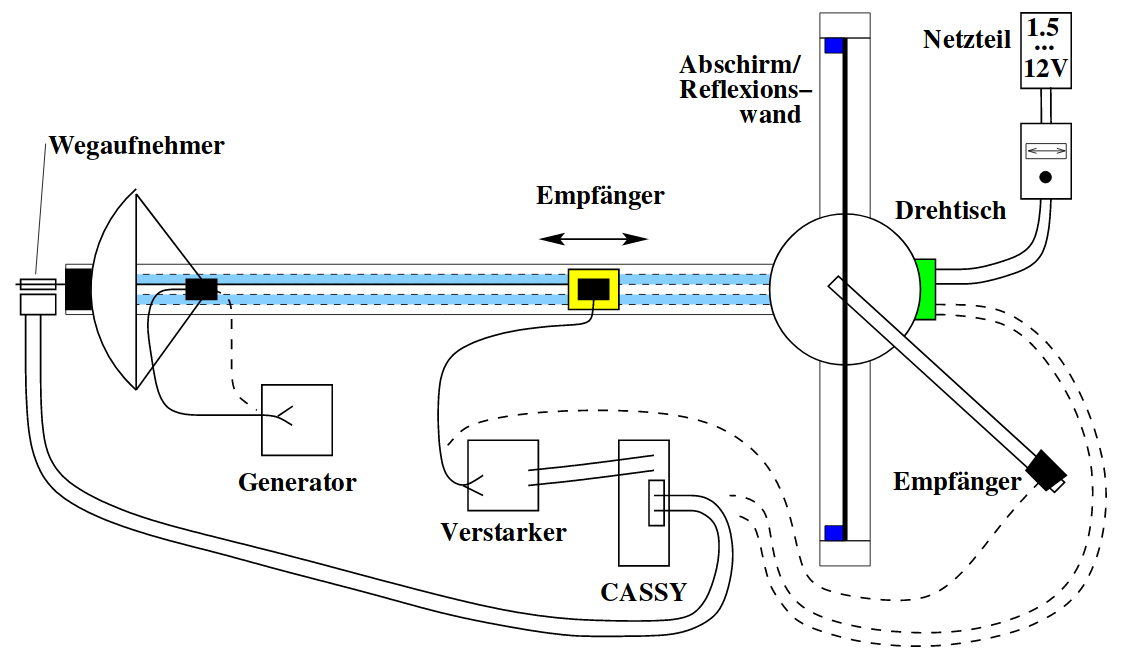
\includegraphics[scale=0.4]{Bilder/versuchsaufbau.png}
	\caption{Versuchsaufbau (Quelle: Versuchshandbuch)}
	\label{versuchsaufbau}
\end{figure}

Der Versuchsaufbau ist in Abb. \ref{versuchsaufbau} dargestellt (bei diesem Teilversuch ohne Parabolspiegel). Ein Piezoelement als Ultraschallsender ist fest auf einer Schiene montiert und mit einem Generator angeschlossen, der den Ultraschallwandler in Resonanzfrequenz anregt. Als Empf"anger dient ebenfalls ein Piezoelement, das auf den Sender gerichtet ist und sich auf der Schiene frei verschieben l"asst. Das Signal des Empf"angers wird "uber einen Verst"arker als Spannung an das Cassy-Ger"at geleitet. Um die Position des Empf"angers zu bestimmen, wird ein Faden von dem Empf"angerstativ "uber das Drehpotentiometer des Wegaufnehmers gef"uhrt und mit einem kleinen Gewicht gespannt. Der Wegaufnehmer gibt die Position des Empf"angers somit als Widerstand aus.

\subsection{Vorversuch: Kalibrierung des Wegaufnehmers}
Zun"achst muss der Wegaufnehmer kalibriert werden. Die L"angenverschiebung $S$ des Empf"angers h"angt linear von der Widerstandsmessung $R$ des Wegaufnehmers ab. Zur Kalibrierung wird der Empf"anger in Schritten von 5cm manuell verschoben, insgesamt 10 Mal, und jeweils der Widerstand aufgenommen. Das Ausmessen erfolgt per Ma\ss band zwischen den F"u\ss en der Piezoelemente.\\
Die Messwerterfassung des Widerstandes erfolgte im Bereich $0..3k\Omega$ und "uber 200ms gemittelt (wie auch im Hauptversuch).\\
Anschlie\ss en wurde eine lineare Regression mit den Daten durchgef"uhrt, wobei die Datens"atze zuerst auf ihren Mittelpunkt verschoben wurden, sodass die Ungenauigkeit auf den Kailbrationsfaktor minimal wird und der y-Achsenabschnitt null.
\begin{equation}
S-\bar{S}=K\cdot(R-\bar{R})
\end{equation}
Wir nehmen Fehler an von 
\begin{align}
\sigma_S &=0.3mm\\
\sigma_R &= \frac{3\text{k}\Omega}{4096\cdot\sqrt{12}}
\end{align}
weil wir die Stative auf ca 1/3mm genau verschieben konnten und wir f"ur den Widerstand den Digitalisierungsfehler des Cassygeräts annehmen.
Wir erhalten den Kalibrierungsfaktor K als Steigung zu $K=16.017\pm0.011cm/k\Omega$. Das $\chi^2/n$ ergibt 1.93. Unter Ber"ucksichtigung der geringen Anzahl an Messpunkten ist dieser Wert ein Hinweis darauf, dass sich die Kalibrierung gut durch die Gerade darstellen l"asst. Der Residuenplot zeigt keine Auff"alligkeiten.
\begin{figure}[H]
	\centering
	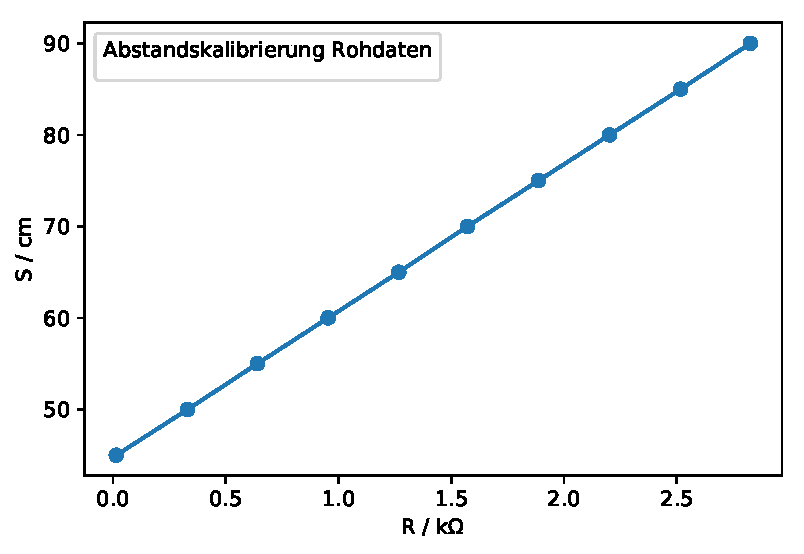
\includegraphics[scale=0.7]{Python/WegaufKal_Rohdaten.pdf}
	\caption{Abstand als Funktion der gemessenen Widerstände des Wegaufnehmers}
	\label{Abstandskal_Rohdaten}
\end{figure}

\begin{figure}[H]
	\centering
	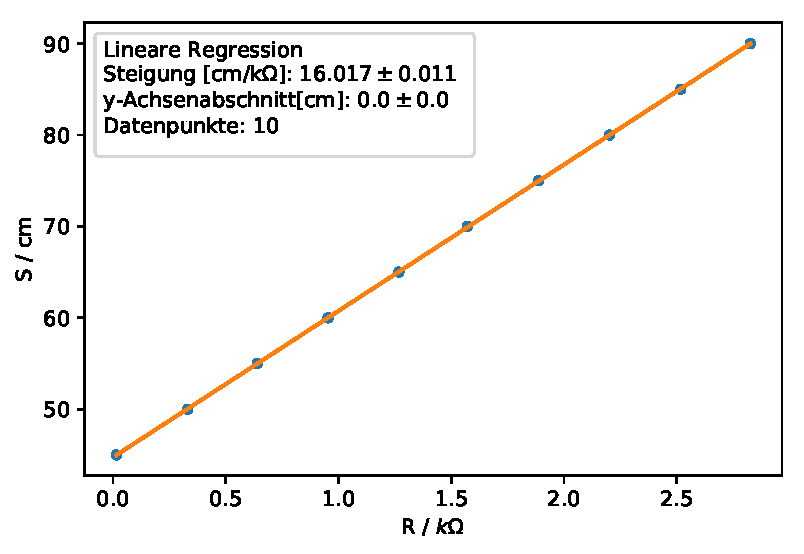
\includegraphics[scale=1]{Python/WegaufKal_LinReg.pdf}
	\caption{Lineare Regression der Kalibrierung des Wegaufnehmers}
	\label{Abstandskal_LinReg}
\end{figure}
\begin{figure}[H]
	\centering
	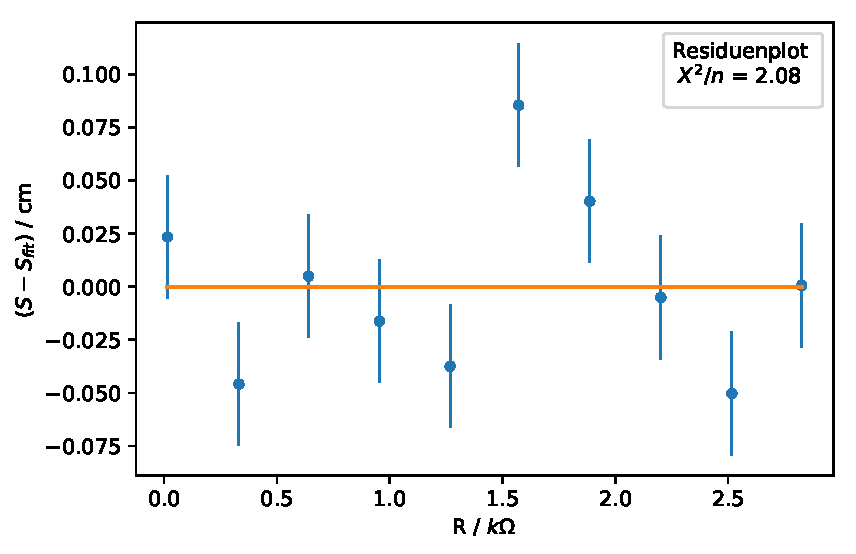
\includegraphics[scale=1]{Python/WegaufKal_Residuen.pdf}
	\caption{Residuenplot der Kalibrierung des Wegaufnehmers}
	\label{Abstandskal_Residuenplot}
\end{figure}





\subsection{Versuchsdurchf"uhrung}
Der Sender sendet eine Kugelwelle aus, sodass die Intensit"at der Schallwelle quadratisch mit der Entfernung f"allt. Der Verst"arker quadriert das Signal des Empf"angers, das wiederum proportional zum Schalldruck ist:
\begin{equation}
U\sim p^a \sim r^{-a}
\end{equation}
mit Erwartung $a=2$ und dem Zusammenhang $I\sim (U/U_0)^{\frac{2}{a}}$
In diesem Versuch wird $a$ berechnet, indem die Spannung des Verst"arkers gegen den Abstand zwischen Sender und Empf"anger $s$ gemessen wird. Dazu wird zuerst der Abstandsoffset zwischen den beiden Piezoelementen mithilfe des Ma\ss bandes bestimmt. Anschlie\ss end schiebt man den Empf"anger langsam von dem Sender und misst die dazukommende Entfernung mithilfe des Wegaufnehmers.\\
Die Messwerterfassung erfolgte folgenderma\ss en:
\begin{table}[H]
	\centering
	\begin{tabular}{|l|c|}
		\hline 
		Messbereich Spannung  & -1 V .. 1 V \\ 
		\hline 
		Messbereich Widerstand Wegaufnehmer & $0\,\text{k}\Omega\ ..\ 3\,\text{k}\Omega$\\ 
		\hline 
		Messwerterfassung Spannung & gemittelt über 200 ms \\ 
		\hline
		Messwerterfassung Widerstand Wegaufnehmer & gemittelt über 200 ms \\ 
		\hline 
		Messwertaufnahme & automatisch, Intervalle von 200 ms \\ 
		\hline 
		Anzahl Messreihen & 3 \\ 
		\hline 
	\end{tabular} 
	\label{tab:MessparameterAllgemein}
\end{table}


\subsection{Versuchsauswertung}
Die Rohdaten wirken, als w"urden die Messwerte stark streuen. Bei genauerer Betrachtung erkennt man jedoch, dass sich stehende Wellen durch Reflexion an weiteren Gegenst"anden im Raum bilden, die zu einer wellenartigen Spannungsverteilung f"uhren.
\begin{figure}[H]
	\centering
	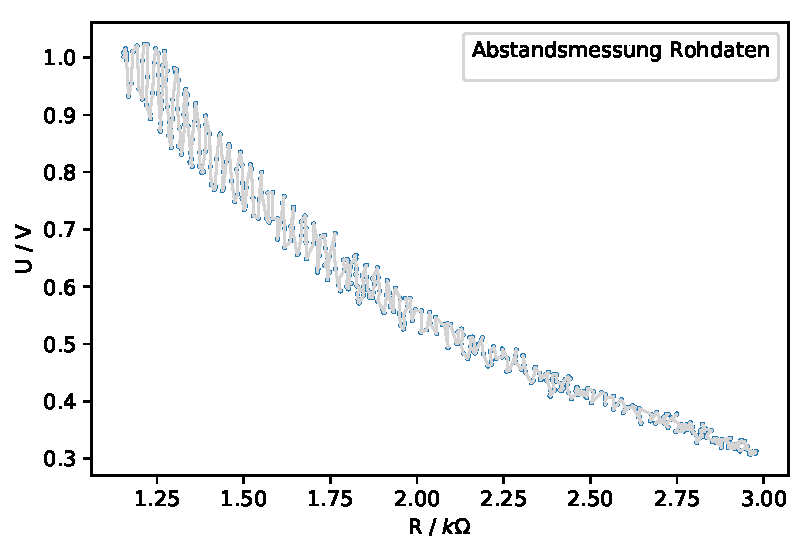
\includegraphics[scale=1]{Python/Abstandsmessung_Rohdaten3.pdf}
	\caption{Rohdaten der Abstandsmessung}
	\label{Abstandskal_Rohdaten}
\end{figure}
Wir messen einen Abstandsoffset von $S_0=25.3cm$ zwischen Sender und Empf"anger bei einem Widerstand des Wegaufnehmers von 1.160k$\Omega$. Als Fehler auf $S_0$ nehmen wir $1mm$ an, weil sich die genaue Position des Piezoelementes im Bauteil nicht genau bestimmen lie\ss. Wir berechnen den Abstand $s$ "uber
\begin{equation}
s=K(R-R_0)+S_0
\end{equation}
Als statistischen Fehler auf $R$ und $R_0$ nehmen wir erneut den Digitalisierungsfehler  von $\sigma_R=3/4096/\sqrt{12}$ an, womit wir f"ur den statistischen Fehler auf $s$ erhalten:
\begin{equation}
\sigma_s(stat)=\sqrt{2}K\sigma_R
\end{equation}
Wir tragen die Spannung doppellogarithmisch auf gegen den Abstand $s$ und f"uhren eine lineare Regression durch. Aus der Steigung erhalten wir den Faktor $-a$.
Der Fehler auf $K$ flie\ss t als systematischer Fehler in den Teilversuch mit ein, wird jedoch bei der linearen Regression zun"achst nicht ber"ucksichtigt. Die Ungenauigkeit auf die Spannung wird wie beim Widersetand mit dem Digitalisierungsfehler des Cassyger"ates angenommen und auf den Logarithmus fortgepflanzt:
\begin{equation}
\sigma_{log(U/V)}=\frac{1V}{U\cdot4096\sqrt{12}}
\end{equation}
Die Fehlerfportpflanzung erfolgt analog f"ur den Abstand.
Die folgenden Graphen zeigen die Ergebnisse der linearen Regression.
\begin{figure}[H]
	\centering
	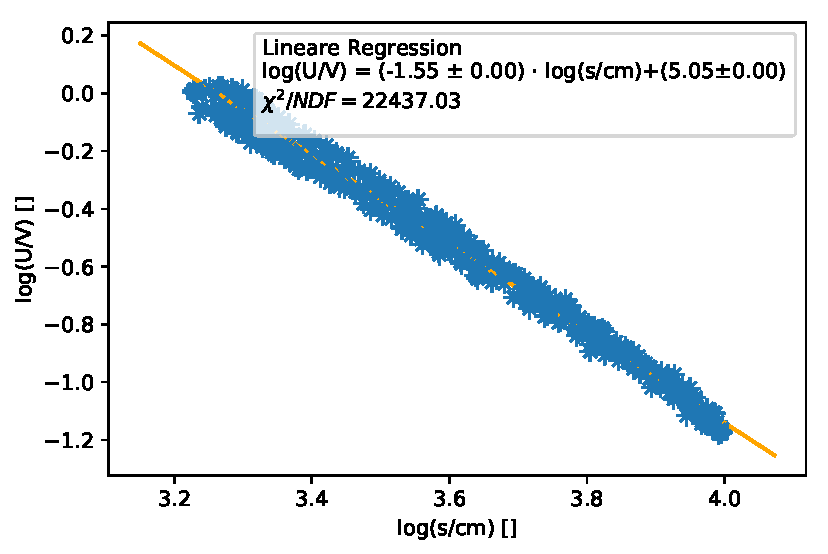
\includegraphics[scale=1]{Python/Abstand3_LinReg.pdf}
	\caption{Lineare Regression der Abstandsmessung}
\end{figure}
\begin{figure}[H]
	\centering
	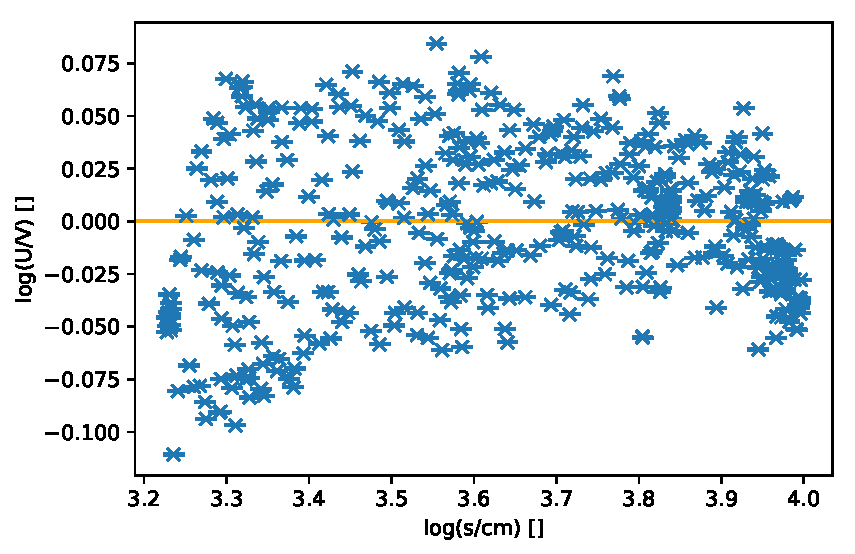
\includegraphics[scale=1]{Python/Abstand3_Residuen.pdf}
	\caption{Residuenplot der Abstandsmessung}
	\label{Abstandsabh_Residuenplot}
\end{figure}
Das $\chi^2/n$ ist mit "uber 20000 sehr gro\ss, was zu erwarten ist, da wir eine wellenartige Verteilung mit einer Gerade anpassen wollen. Die Graphen zeigen jedoch, dass die Gerade durchaus den durchschnittlichen Verlauf der Intensit"at wiedergibt. Wir erhalten einen Wert von $a=1.55$, wobei der Fehler auf $a$ aus der linearen Regression unbrauchbar ist. Um trotzdem eine sinnvolle Breite f"ur $a$ zu berechnen, werden zwei weitere Messreihen analog ausgewertet. Die Werte f"ur $a$ dieser Messreihen lauten $a=1.60$ und $a=1.53$. Wir berechnen den ungewichteten Mittelwert dieser drei Werte von $a$ und die empirische Standardabweichung als Ma\ss\  f"ur die Unsicherheit. Um den systematischen Fehler auf $a$ zu erhalten, wird die gesamte Rechnung mit um $\sigma_{S_0}$ und $\sigma_{K}$ verschobenem $s$ wiederholt, und die Differenz von $a$ zum urspr"unglichen $a$ als systematischen Fehler angerechnet. Insgesamt erh"alt man so:
\begin{equation}
a=1.561\pm0.038(stat)\pm0.004(sys)
\end{equation}
Der Wert weicht von der Erwartung $a=2$ ab, weil die Piezoelemente wom"oglich keine idealen Kugelwellen aussenden und die Messung durch Reflexion an umliegeneden W"anden gest"ort wird.


\section{Stehende Wellen}

\subsection{Versuchsaufbau}
Ziel dieses Versuchs ist die Bestimmung der Wellenl"ange durch das Vermessen von stehenden Wellen, die durch Reflexion von ebenen Wellen an einer Wand entstehen.
Zur Erzeugung der ebenen Wellen wird ein Parabolspiegel an die Schiene gebaut und der Sender im Brennpunkt und auf den Spiegel zeigend positioniert. Am Schienenende wird eine Wand montiert und der verschiebbare Empf"anger Richtung Wand ausgerichtet. Wie im vorherigen Versuch l"asst sich die Position des Empf"angers mit dem Wegaufnehmer bestimmen.

\subsection{Versuchsdurchf"uhrung}
Der Empf"anger wird auf der Schiene langsam verschoben und die Spannung des Verst"arkers als Funktion des Widerstandes am Wegaufnehmer gemessen. Die genaue Entfernung zur Wand wird bei dem Versuch nicht ben"otigt, sodass kein Abstandsoffset in die Berechnung mit einflie\ss t.
Die Messwerterfassung erfolgt identisch zum vorherigen Versuch und es werden wieder drei Messreihen durchgef"uhrt.

\subsection{Versuchsauswertung}
Die Spannung wird gegen den Widerstand graphisch aufgetragen und es ist klar erkennbar, dass sich stehende Wellen mit B"auchen (Maxima) und Knoten (Minima) in gleichen Abst"anden ausbilden. Wir w"ahlen  f"ur jede Messung einen m"oglichst gro\ss en Bereich zwischen zwei Knoten und z"ahlen die Knoten $N$ in diesem Intervall, wobei wir den ersten nicht mitz"ahlen. 

\begin{figure}[H]
	\centering
	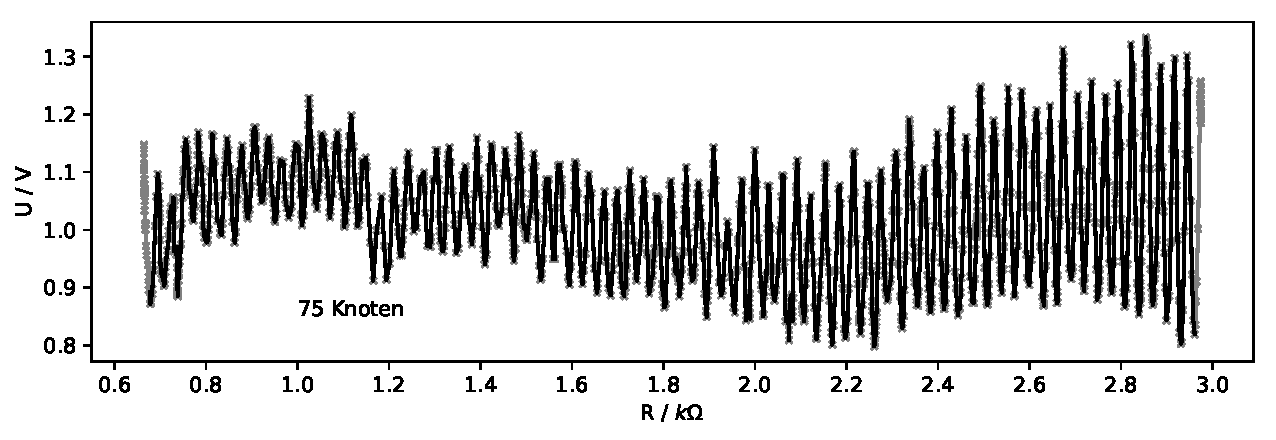
\includegraphics[scale=0.8]{Python/stehwel1.pdf}
	\caption{Stehende Welle: Messung 1. Der dunkelunterlegte Bereich enth"alt 75 halbe Wellenl"angen. (Der erste Knoten wird bei der Z"ahlung nicht mitgez"ahlt.)}
\end{figure}

Die Wellenl"ange $\lambda$ erhalten wir durch
\begin{equation}
\lambda=K\Delta R\frac{2}{N}
\end{equation}
$\Delta R=R_N-R_0$ ist die Widerstandsdifferenz zwischen dem letztem und dem 0. Knoten. Auf die genaue Position der Knoten nehmen wir eine Ungenauigkeit von $\sigma_R=0.003k\Omega$ an, da es pro Knotenpunkt nur wenige Messwerte gibt und sich bei Betrachtung der einzelnen Widerstandswerte der Knotenpunkt ca. auf diese Gr"o\ss enordnung genau bestimmen lie\ss. Damit erhalten wir einen statistischen Fehler von
\begin{equation}
\sigma_{\lambda}(stat)=\sqrt{2}K\frac{2}{N}\sigma_{R}.
\end{equation}
Der Fehler auf $K$ f"uhrt zu einem systematischen Fehler in der Wellenl"ange.
\begin{equation}
\sigma_{\lambda}(sys)=\Delta R\frac{2}{N}\sigma_{K}.
\end{equation}

\begin{figure}[H]
	\centering
	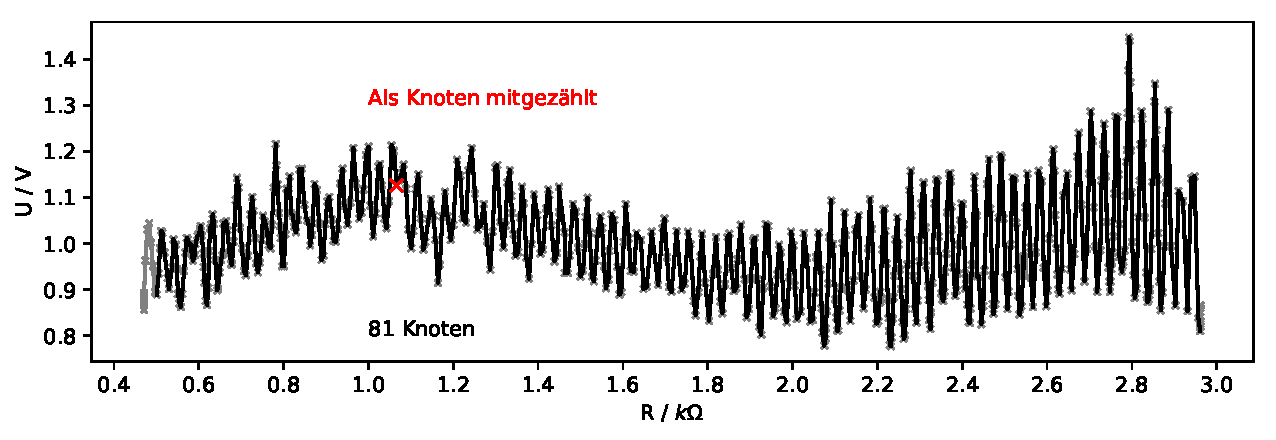
\includegraphics[scale=0.8]{Python/stehwel2.pdf}
	\caption{Stehende Welle: Messung 2.}
\end{figure}

\begin{figure}[H]
	\centering
	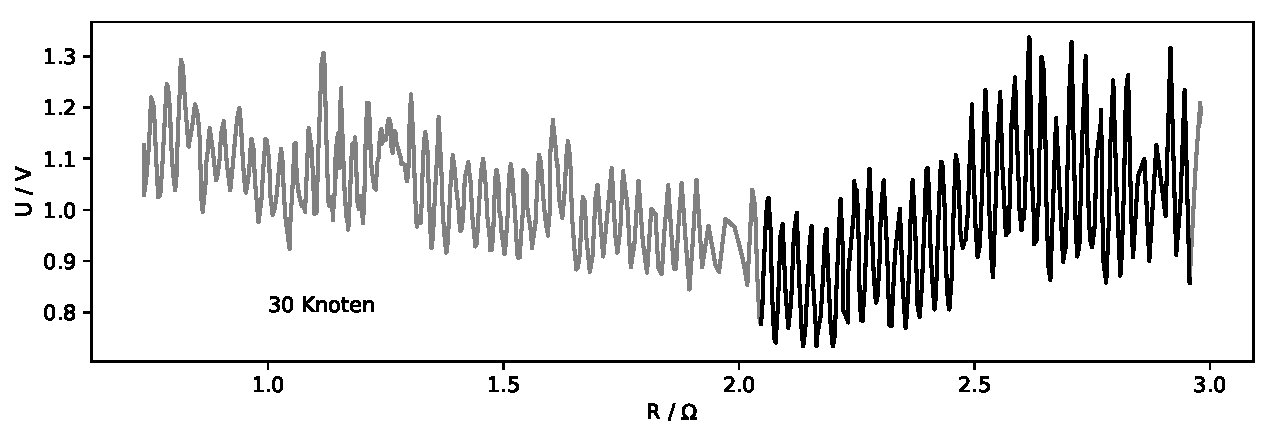
\includegraphics[scale=0.8]{Python/stehwel3.pdf}
	\caption{Stehende Welle: Messung 3, erste Z"ahlung}
\end{figure}

\begin{figure}[H]
	\centering
	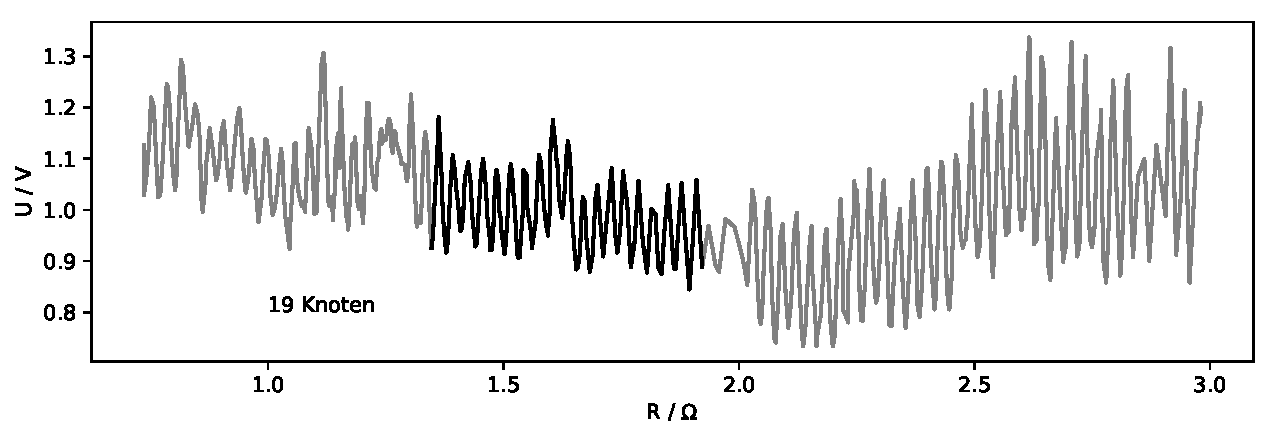
\includegraphics[scale=0.8]{Python/stehwel4.pdf}
	\caption{Stehende Welle: Messung 3, zweite Z"ahlung}
\end{figure}

Bei der dritten Messung gibt es mehrere Bereiche, in denen nicht erkennbar ist, ob dort ein Knotenpunkt entsteht. Teilweise liegt das daran, dass der Empf"anger zu schnell bewegt wurde. Wir entscheiden uns, zwei Bereiche getrennt auszuwerten, in denen die Anzahl an Knotenpunkten eindeutig gez"ahlt werden kann. Insgesamt erhalten wir so vier Berechnungen der Wellenl"ange, die in folgender Tabelle zusammengefasst sind.
\begin{table}[H]
	\centering
	\begin{tabular}{|l|l|l|l|}
		\hline 
		& $\lambda$[cm]&$\sigma_{\lambda}(stat)$[cm]&$\sigma_{\lambda}(sys)$[cm]\\ 
		\hline 
		Messung 1&0.9751&0.0018&0.0006\\
		\hline
		Messung 2&0.9729&0.0017&0.0006\\
		\hline
		Messung 3&0.9722&0.0045&0.0006\\
		\hline
		Messung 4&0.9686&0.0072&0.0006\\
		\hline
	\end{tabular} 
\end{table}
Da die Messungen innerhalb ihrer statistischen Fehler "ubereinstimmen, berechnen wir das gewichtete Mittel und erhalten:
\begin{equation}
\lambda=0.9736\pm0.0012(stat)\pm0.0006(sys)\ cm
\end{equation}

\section{Beugung am Einzelspalt und Doppelspalt}

\subsection{Versuchsaufbau}
Ziel dieses Versuchs ist es die Intensit"atsverteilung hinter einem Einzel- oder Doppelspalt in Abh"angigkeit des Winkels $\phi$ zur Einfallsrichtung zu bestimmen. Der Aufbau des Senders mit dem Parabolspiegel zur Erzeugung ebener Wellen aus dem vorherigen Versuch bleibt bestehen. Der Empf"anger dagegen wird dagegen an einem schwenkbaren Dreharm hinter der Reflexionswand befestigt (Der Aufbau entspricht den gestrichelten Linien von Abb. \ref{versuchsaufbau}). In die Reflexionswand lassen sich mithilfe von verschiebbaren Metallplatten Einzelspalten und Doppelspalten unterschiedlicher Breite einbauen. Der Drehtisch, an dem der Dreharm befestigt ist, l"asst sich mit einem Motor drehen und ist mit einem Drehpotentiometer verbunden, der somit als Winkelaufnehmer wirkt. 

\subsection{Vorversuch: Kalibrierung des Winkelaufnehmer}
Zun"achst muss in einem Vorversuch der Winkelaufnehmer kalibriert werden. Der Winkel $\phi$ h"angt linear von der Widerstandsmessung $R$ des Winkelaufnehmers ab. Zur Kalibrierung wird der Dreharm in Schritten von $\ang{10}$ von $\ang{-80}$ bis $\ang{80}$ manuell gedreht und jeweils der Widerstand aufgenommen. Die Winkel werden an dem Drehtisch abgelesen. Die Messwerterfassung des Widerstandes erfolgte im Bereich $0..10k\Omega$ und "uber 200ms gemittelt.\\
Analog zur Kalibration des Wegaufnehmers erwartet man einen linearen Zusammenhang zwischen dem gemessenen Widerstandswert $R$ und dem Drehwinkel $\phi$, sodass man wieder eine lineare Regression der Art

\begin{equation}
	R-\bar{R}=K\cdot(\phi-\bar{\phi})
\end{equation}

durchführen kann. Als Fehler wurden hier folgende Werte genommen:
\begin{center}
	$\sigma_R = \SI{0.005}{k \Omega}$\\
	$\sigma_{\phi} = 0.5^\circ$
\end{center}
Die Ergebnisse der Regression sind in der Abb. \ref{fig:winkelkalib} dargestellt:

\begin{figure}[H]
	\centering
	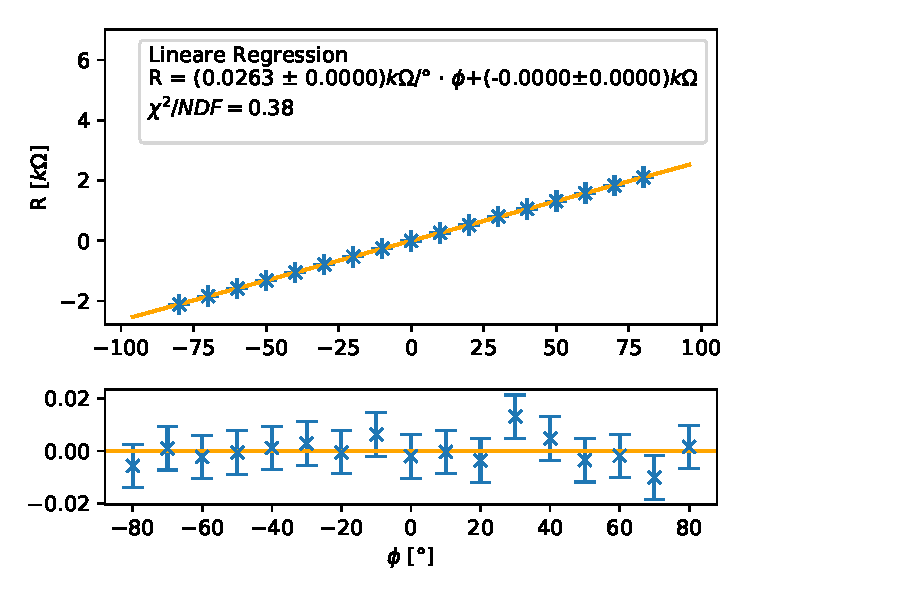
\includegraphics[width=0.7\linewidth]{Rohdaten/Images/Winkelkalib}
	\caption{Lineare Regression des Winkelaufnehmers}
	\label{fig:winkelkalib}
\end{figure}

Als Ergebnis der Regression erhält man einen $K$-Wert von $(0.02633\pm0.00007)k\Omega/^\circ$. Dieses Ergebnis wurde auf $\phi$ umgestellt (man misst den Widerstand $R$), sodass es einen Umrechnungsfaktor von $K^{-1} =(37.9795\pm0.1006)^\circ/k\Omega$ ergibt.

%Auffallend ist im Residuenplot das kleine $\chi^2/n_{ndf}$...



\subsection{Versuchsdurchf"uhrung}
Zuerst werden die Metallplatten mthilfe eines Ma\ss bandes auf die zu untersuchende Spaltbreite eingestellt.
Als n"achstes wird der Empf"anger auf $\pm\ang{80}$ geschoben und (beim Einzelspalt der Breite d=3cm und beim Doppelspalt) der Motor des Drehtisches gestartet, sodass der Empf"anger langsam um den Drehtisch schwenkt. Im Falle des Einzelspalts der Breite d=4cm wurden die Werte per Hand aufgenommen. Die Messung wird wiederholt, indem auch der R"uckweg aufgezeichnet wird.\\
Die Messwerterfassung erfolgte folgenderma\ss en:
\begin{table}[H]
	\centering
	\begin{tabular}{|l|c|}
		\hline 
		Messbereich Spannung (Dop.-Spalt, Einzelspalt 4cm)  & -1 V .. 1 V \\ 
		\hline 
		Messbereich Spannung (Einzelspalt 3cm bzw. 4cm)  & -0.3 V .. 0.3 V \\ 
		\hline 
		Messbereich Widerstand Winkelaufnehmer & $0\,\text{k}\Omega\ ..\ 10\,\text{k}\Omega$\\ 
		\hline 
		Messwerterfassung Spannung & gemittelt über 200 ms \\ 
		\hline
		Messwerterfassung Widerstand Wegaufnehmer & gemittelt über 200 ms \\ 
		\hline 
		Messwertaufnahme & automatisch, Intervalle von 200 ms \\ 
		\hline 

	\end{tabular} 
	\label{tab:MessparameterAllgemein}
\end{table}

\subsection{Versuchsauswertung}
Unser Ziel ist es, die Spannung des Verstärkers gegen den Widerstand des Winkelaufnehmers aufzuzeichnen, und die Ergebnisse mit der theoretischen Erwartung zu vergleichen. Dafür werden die gemessenen Spannungswerte über die Proportionalität $I\propto U^{\frac{2}{a}}$ umgerechnet und die Lagen der Maxima der so erhaltenen Intensitätsverteilung bestimmt. Mit den so gewonnenen Informationen können wir auch die Wellenlänge $\lambda$ des Ultraschalls über die folgenden Beziehungen berechnen:
\begin{align}
	\lambda &= \frac{\pi}{4.49341\footnotemark}b \cdot \sin(\phi),&\, \text{für einen Einzelspalt der Breite b}
	\label{eq:lambda2}\\
	\lambda &= d \cdot \sin(\phi),&\, \text{für einen Doppelspalt mit Spaltabstand d}
	\label{eq:lambda1}
\end{align}
\footnotetext{der Faktor 4.49341 kommt durch $((\sin(x)/x)^2)'=0  \Rightarrow x = \tan(x)$ zustande (für die Maxima erster Ordnung)}
Die Rohdaten (mit den umgerechneten Widerstandswerten) zweier Beispielmessungen sind in der Abb. \ref{fig:rohdaten} dargestellt. Man erkennt sofort, dass die Peaks unscharf erscheinen, sodass die Unsicherheiten auf die Maxima unvermeidlich groß wird. Außerdem sieht man auch, dass die Verteilung gegen die Nullage verschoben ist, sodass sie zuerst zentriert werden soll, um sie mit der theoretischen Vorhersage zu vergleichen.
\begin{figure}[H]
	\centering
	\begin{subfigure}{.5\textwidth}
		\centering
		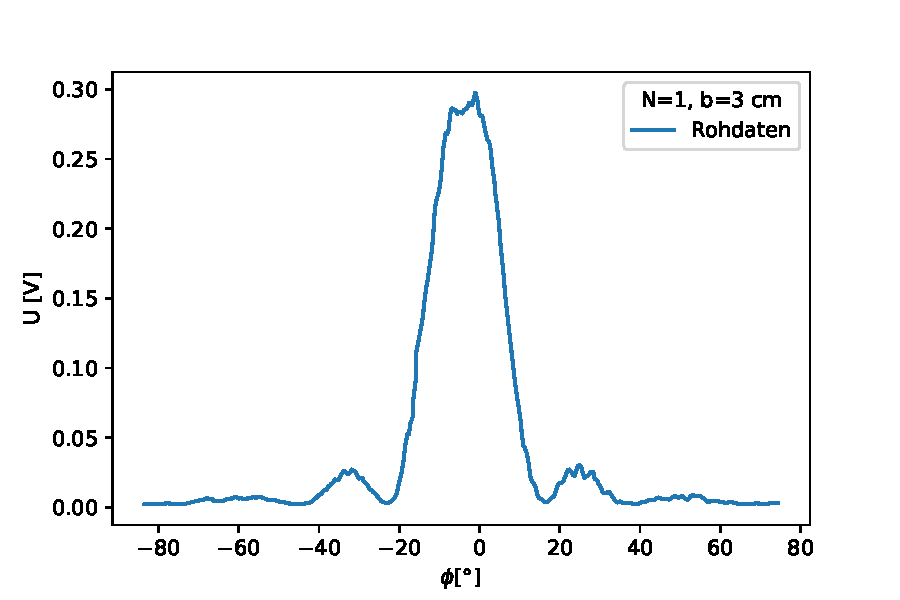
\includegraphics[width=0.9\linewidth]{Rohdaten/Images/einzelspalt_roh_3_3}
	\end{subfigure}%
	\begin{subfigure}{.5\textwidth}
		\centering
		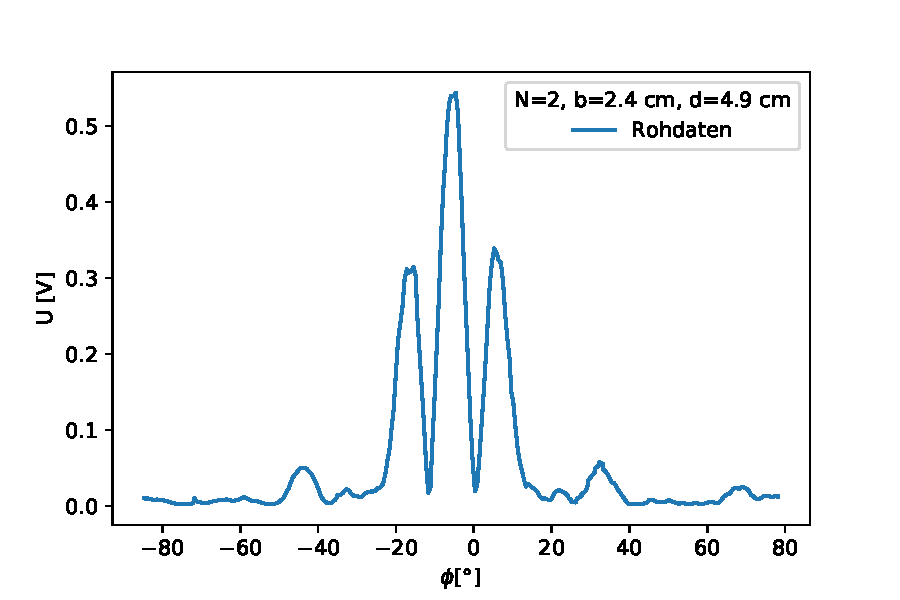
\includegraphics[width=0.9\linewidth]{Rohdaten/Images/doppelspalt_roh_2}
	\end{subfigure}
	\caption{Rohdaten der Spannungsmessung}
	\label{fig:rohdaten}
\end{figure}
Aus diesen (insgesamt 11) Graphen wurden zuerst die Lagen $\phi_1,  \phi_2$ der Maxima erster Ordnung mittels der Python-Bibliothek scipy bestimmt. Um die Graphen zu zentrieren, wurden alle Daten mit $(\phi_1+\phi_2)/2$ verschoben, sodass diese Maxima symmetrisch um den Nullpunkt liegen. Die Plots der gleichen verschobenen Rohdaten sind in Abb. \ref{fig:daten_mit_theo} dargestellt.

\begin{figure}[H]
	\centering
	\begin{subfigure}{.5\textwidth}
		\centering
		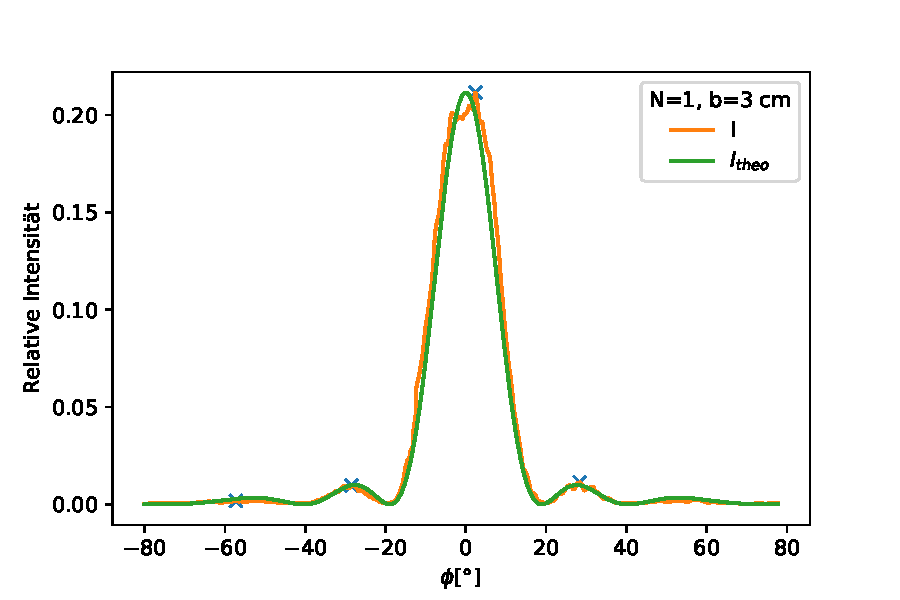
\includegraphics[width=0.9\linewidth]{Rohdaten/Images/einzelspalt_3_3}
	\end{subfigure}%
	\begin{subfigure}{.5\textwidth}
		\centering
		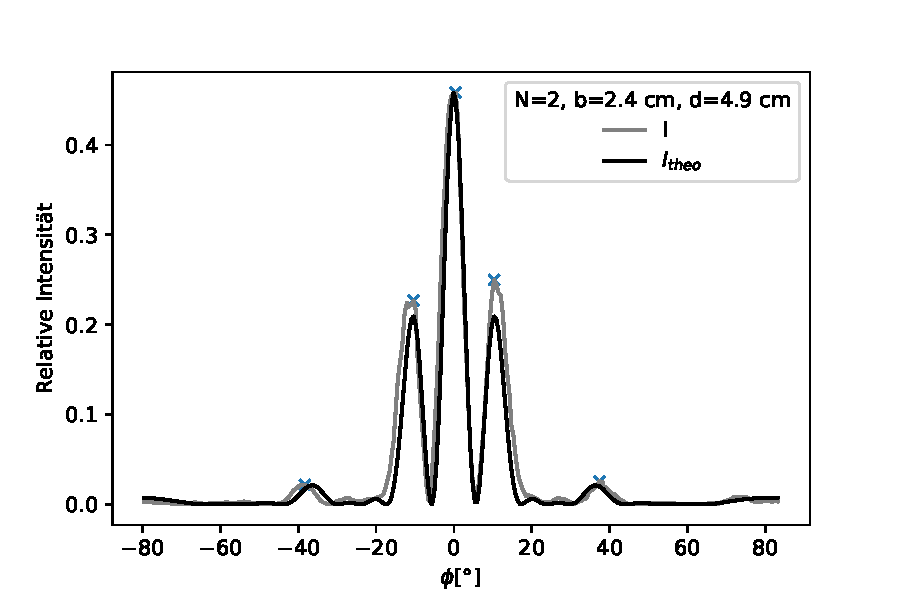
\includegraphics[width=0.9\linewidth]{Rohdaten/Images/doppelspalt_2}
	\end{subfigure}
	\begin{subfigure}{.5\textwidth}
		\centering
		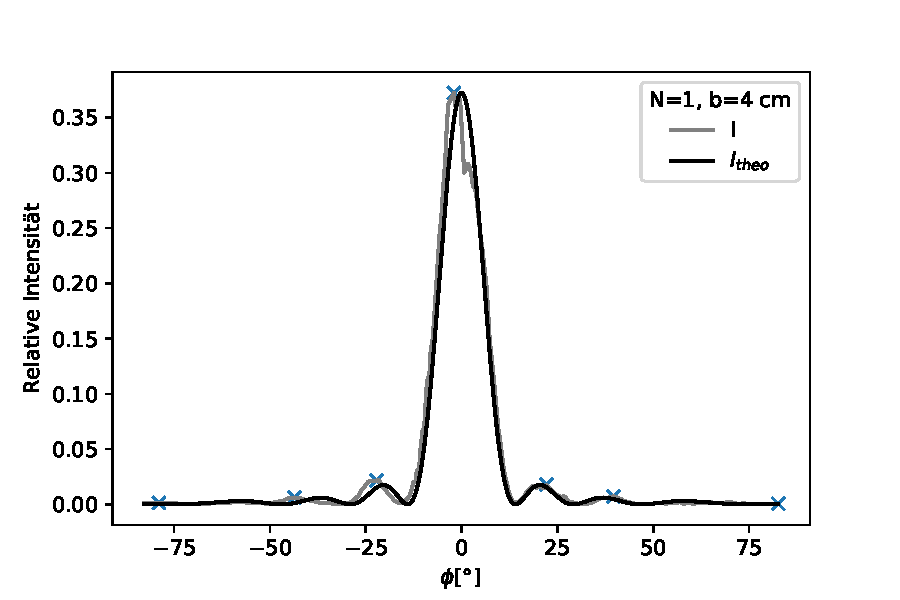
\includegraphics[width=0.9\linewidth]{Rohdaten/Images/einzelspalt_4_3}
	\end{subfigure}%
	\begin{subfigure}{.5\textwidth}
		\centering
		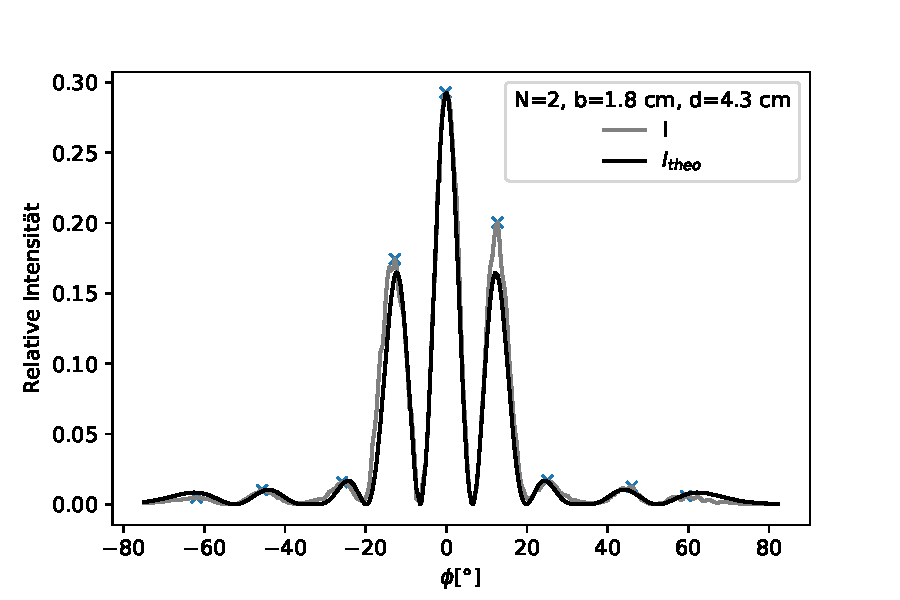
\includegraphics[width=0.9\linewidth]{Rohdaten/Images/doppelspalt_3}
	\end{subfigure}
	\caption{Rohdaten der Spannungsmessung}
	\label{fig:daten_mit_theo}
\end{figure}

Durch Zusammenfassen der einzelnen Messungen erhält man in der folgenden Tabelle dargestellten Werte.\\
\begin{table}[H]
	\centering
	\begin{tabular}{|l|c|c|}
		\hline 
		Messkonfiguration& Gemessener Wert & Theoretischer Wert \\ 
		\hline 
		Einzelspalt d=3cm &(28,4$\pm$0,95)$^\circ$&27,69$^\circ$ \\ 
		\hline 
		Einzelspalt d=4cm &(21,245$\pm$0,95)$^\circ$ &20,4$^\circ$ \\ 
		\hline 
		Doppelspalt d=4,9cm, b=2,4cm&(10,455$\pm$1,34)$^\circ$ &11.47$^\circ$ \\ 
		\hline 
		Doppelspalt d=4,3cm, b=1,8cm&(12,74$\pm$1,9)$^\circ$ &13,1$^\circ$ \\
		\hline 
	\end{tabular}
	\caption{Zusammenfassung der gemessenen Maxima}
\end{table}
Man erkennt, dass alle der gemessenen Werte im 1$\sigma$-Bereich der theoretischen Vorhersage liegen. Allerdings gibt es Abweichungen in der Intensität, die sich unter Anderem auf Störeffekte (Reflexion an herumliegenden Gegenständen) zurückführen lassen, was durch eine Rauschmessung hätte korrigiert werden können.\\
Aus der Lage der zuvor erwähnten Maxima kann man mithilfe der Gl. \ref{eq:lambda1} und der Gl. \ref{eq:lambda2} die Wellenlänge $\lambda$ bestimmen. Der Fehler $\sigma_\lambda$ wurde mittels Fehlerfortpflanzung bestimmt (wobei $\sigma_d=\sigma_b=1mm/\sqrt{12}$)
\begin{equation*}
	\sigma_{\lambda 1}^2 = \left(\frac{\pi}{4.49341}\right)^2 \cdot \left[(\sin(\phi)\sigma_b)^2+(b\cos(\phi)\sigma_\phi)^2\right]
\end{equation*}
\begin{equation*}
	\sigma_{\lambda {2}}^2 = \left[(\sin(\phi)\sigma_d)^2+(d\cos(\phi)\sigma_\phi)^2\right],
\end{equation*}
sodass man durch Kombination aller Messungen erhält
\begin{equation}
	\lambda = (0.9961 \pm 0.0171) cm.
\end{equation}
Dieser Wert liegt im 1,3$\sigma$-Bereich des im Abschnitt 3.3 erhaltenen Werts. Dieses Ergebnis lie\ss e sich verbessern, indem man die Extrema höherer Ordnungen mitbetrachtet, sofern in der Messung sichtbar.


\section{Zusammenfassung}
Bei der Abstandsmessung konnte der Exponentialfaktor $a$ zur Umrechnung der gemessenen Spannung $U$ zur Intensit"at der Schallwelle $I\sim(U/U_0)^{2/a}$ bestimmt werden zu
\begin{equation}
a=1.561\pm0.038(stat)\pm0.004(sys).
\end{equation}
Die Wellenl"ange konnte zum einen "uber die Vermessung von stehenden Wellen bestimmt werden, zum anderen "uber die Auswertung der Intensit"atsverteilungen hinter Einzelspalten und Doppelspalten.
\begin{equation}
\lambda_{Stehende Welle}=0.9736\pm0.0012(stat)\pm0.0006(sys)\ cm
\end{equation}
\begin{equation}
\lambda_{Beugung} = (0.9961 \pm 0.0171) cm.
\end{equation}
St"oreffekte treten vor allem durch die Reflexion der Schallwelle an Raumw"anden und Gegenst"anden auf.

\end{document}